\chapter{Design requirements}

In this chapter the requirement for the TID sensor will be presented.

Sensor is designed to be flown on-board of PW-Sat2 satellite. Therefore it should be designed for its particular requirements. In addition, it should be designed having in mind active space standard and launcher requirements.


\section{PW-Sat2 mission}
	Presented sensor is scheduled to be launched on PW-Sat2 satellite \cite{PW-Sat2URL}. Therefore it should be designed especially for this particular type of mission. In this section PW-Sat2 mission will be presented. On fig. \ref{PW-Sat_render_01} exploded render is presented.
	
	\begin{figure}[h]
		\centering
		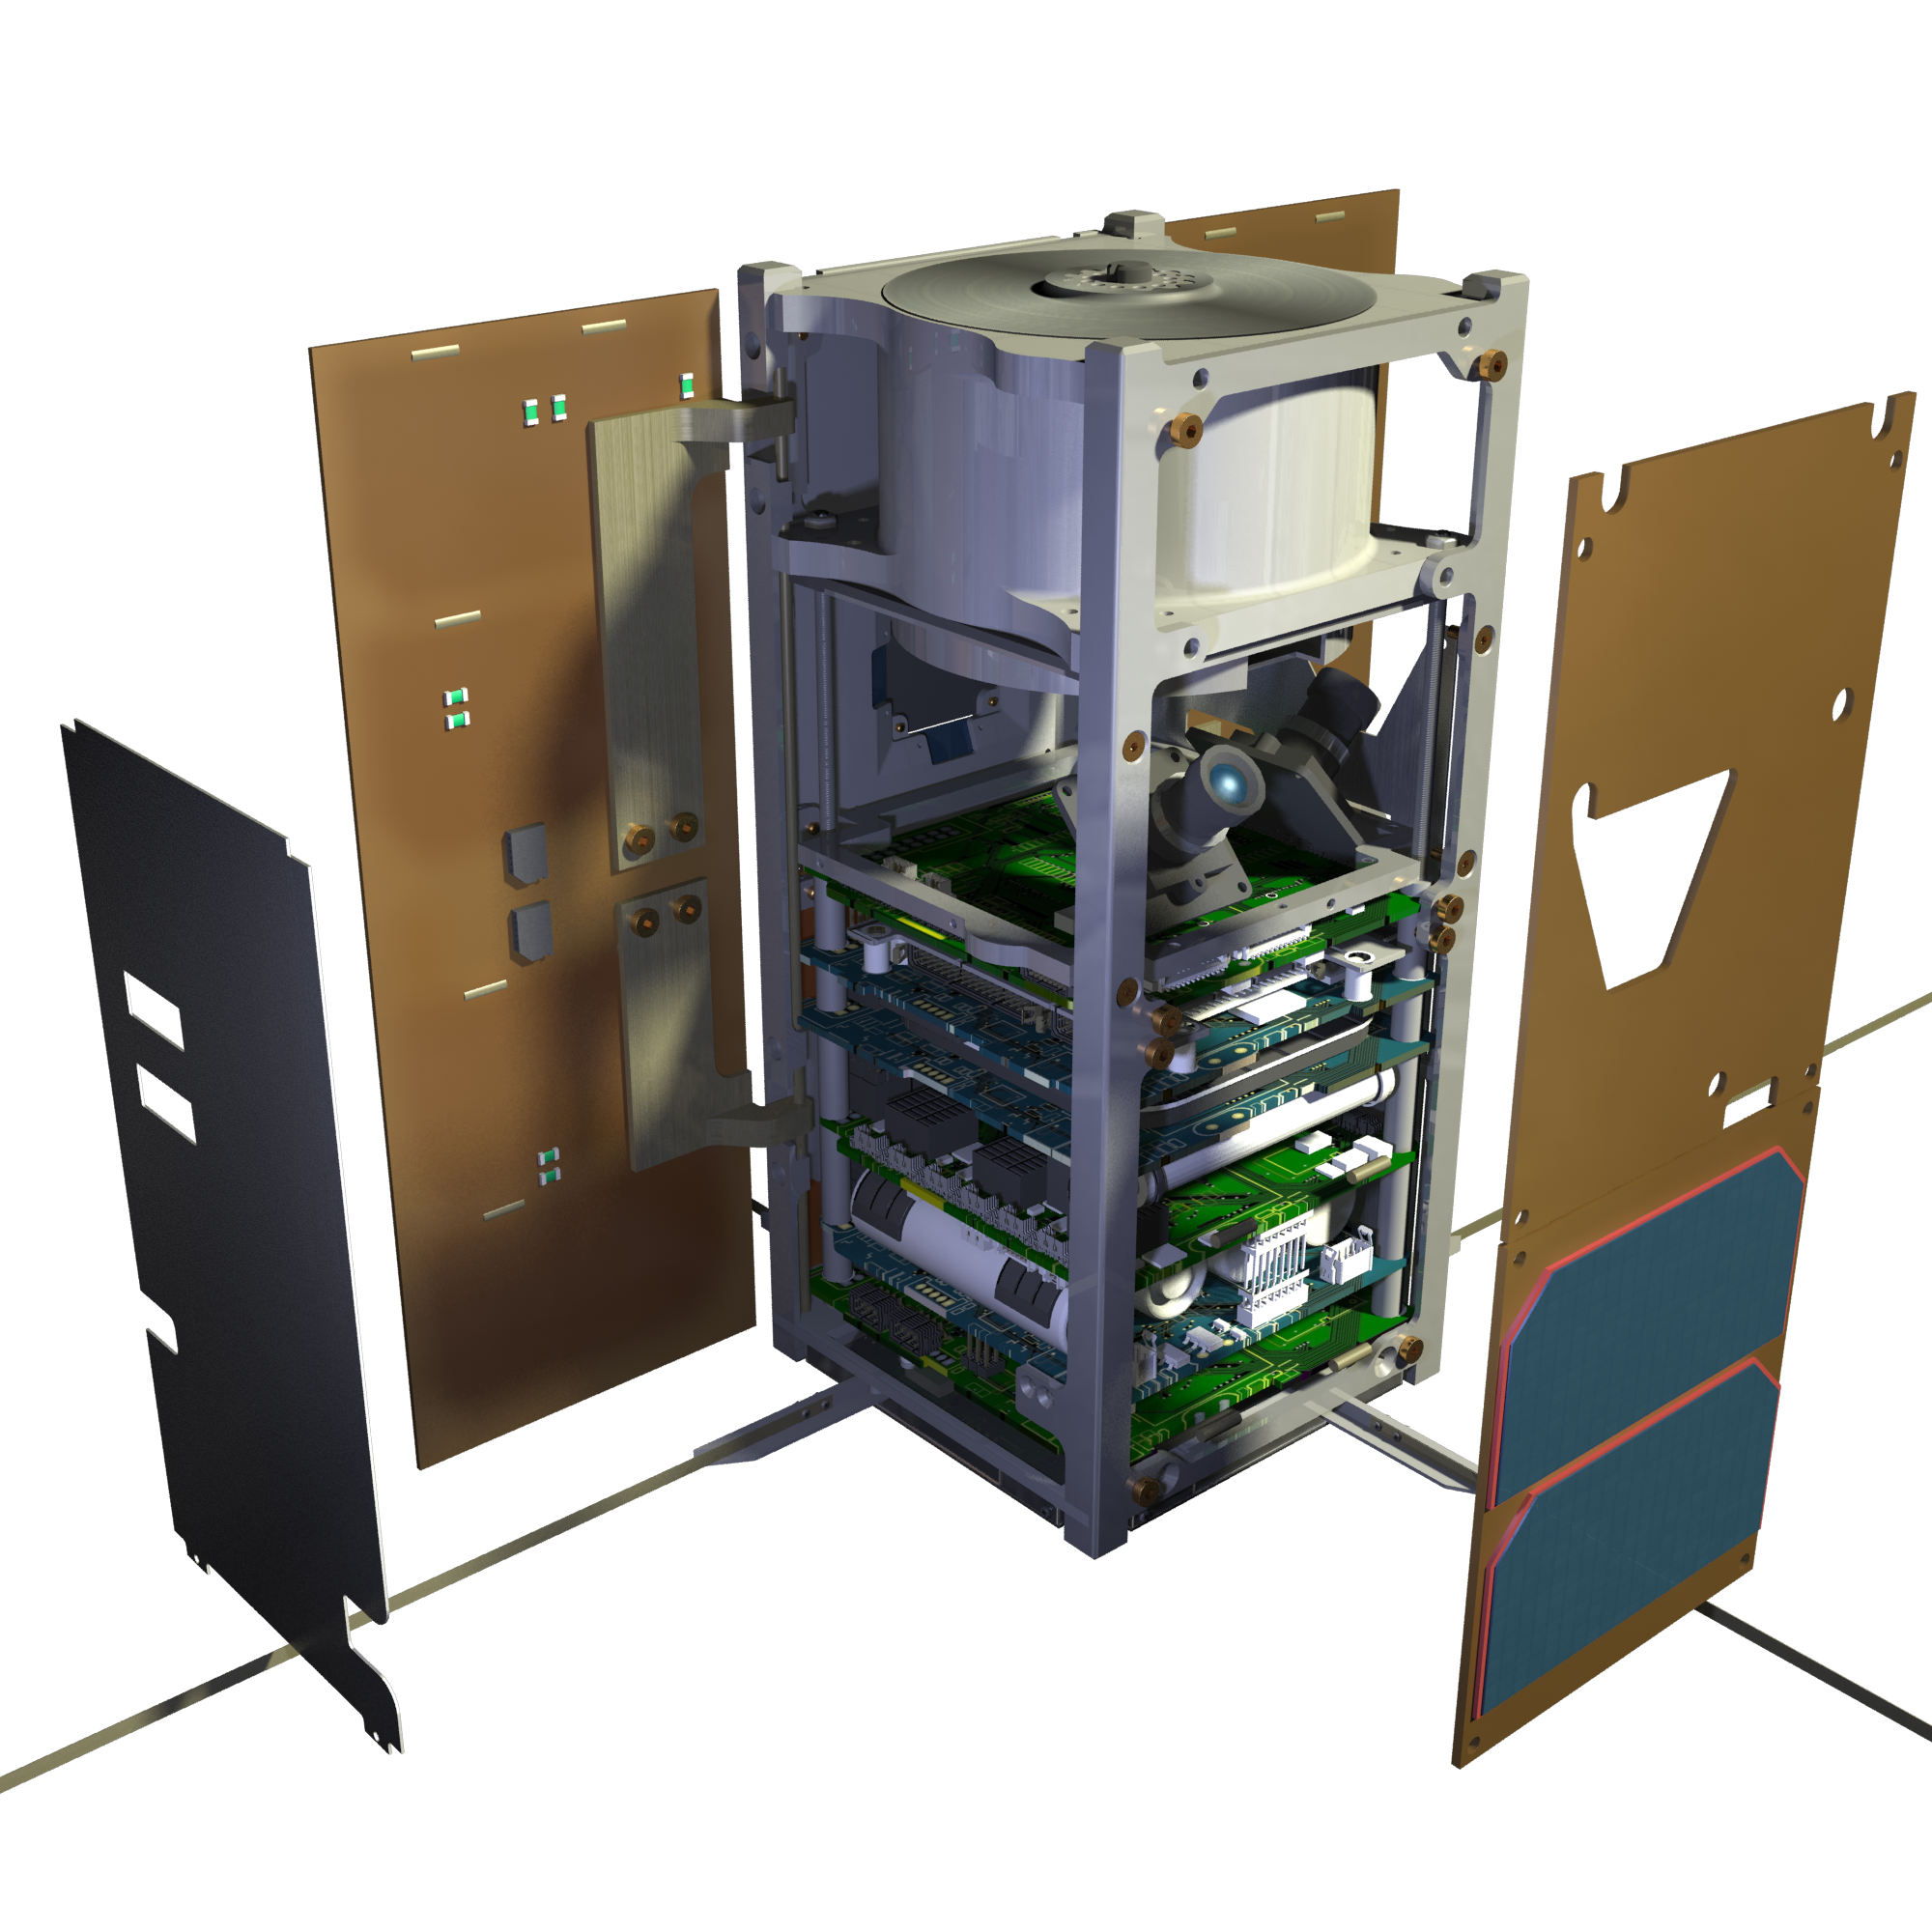
\includegraphics[width=0.5\paperwidth]{img/PW-Sat2_render_01.png}
		\caption{PW-Sat2 render (by M. Świetlik)}
		\label{PW-Sat_render_01}
	\end{figure}

	PW-Sat2 is scheduled to be launched on Falon9 rocket from SpaceX company in Q4 2017.
	
	\begin{figure}[H]
		\centering
		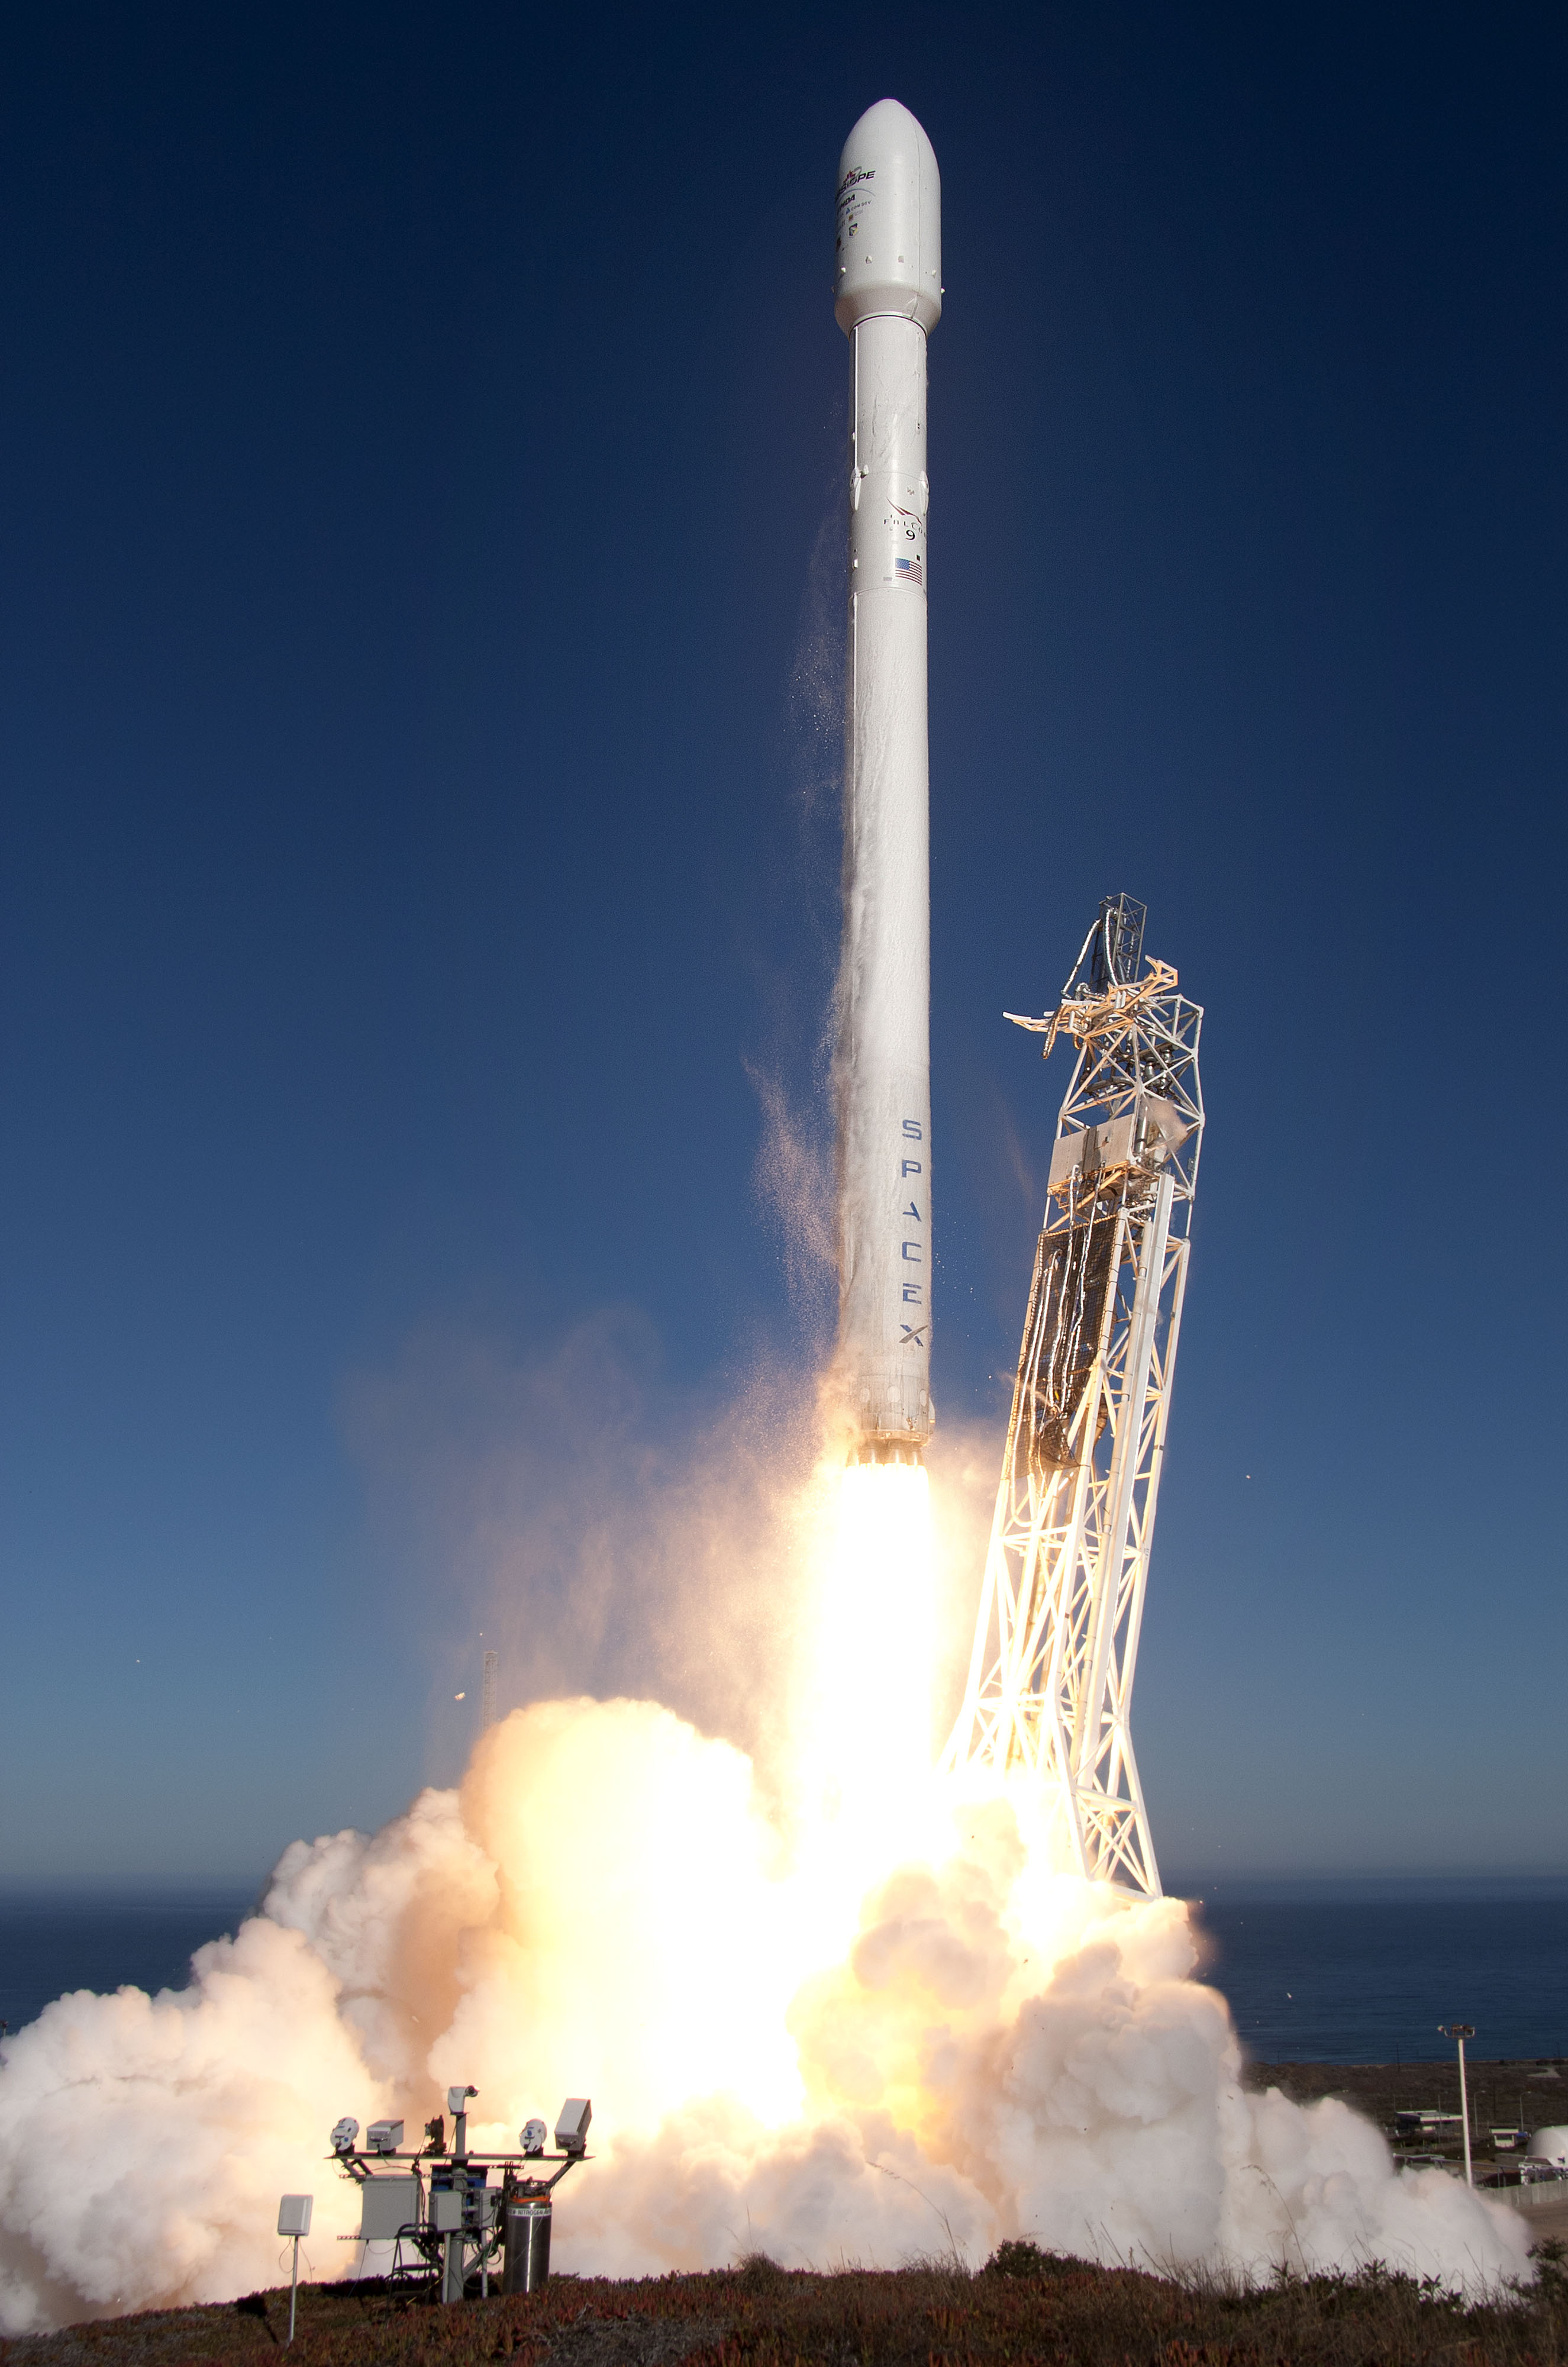
\includegraphics[width=0.3\paperwidth]{img/Falcon9.jpg}
		\caption{Falcon9 rocket. Source: \url{www.spacex.com}}
		\label{PW-Sat_render_01}
	\end{figure}
	
	
\subsection{Primary mission}
	Primary mission of PW-Sat2 is to test deorbiting sail. Its purpose is to increase atmospheric drag and shorten satellite life. This method of deorbitation could be easy way to reduce space debris on LEO. Render of PW-Sat2 with opened sail is on \ref{PW-Sat_render_sail}.
	
	\begin{figure}[H]
		\centering
		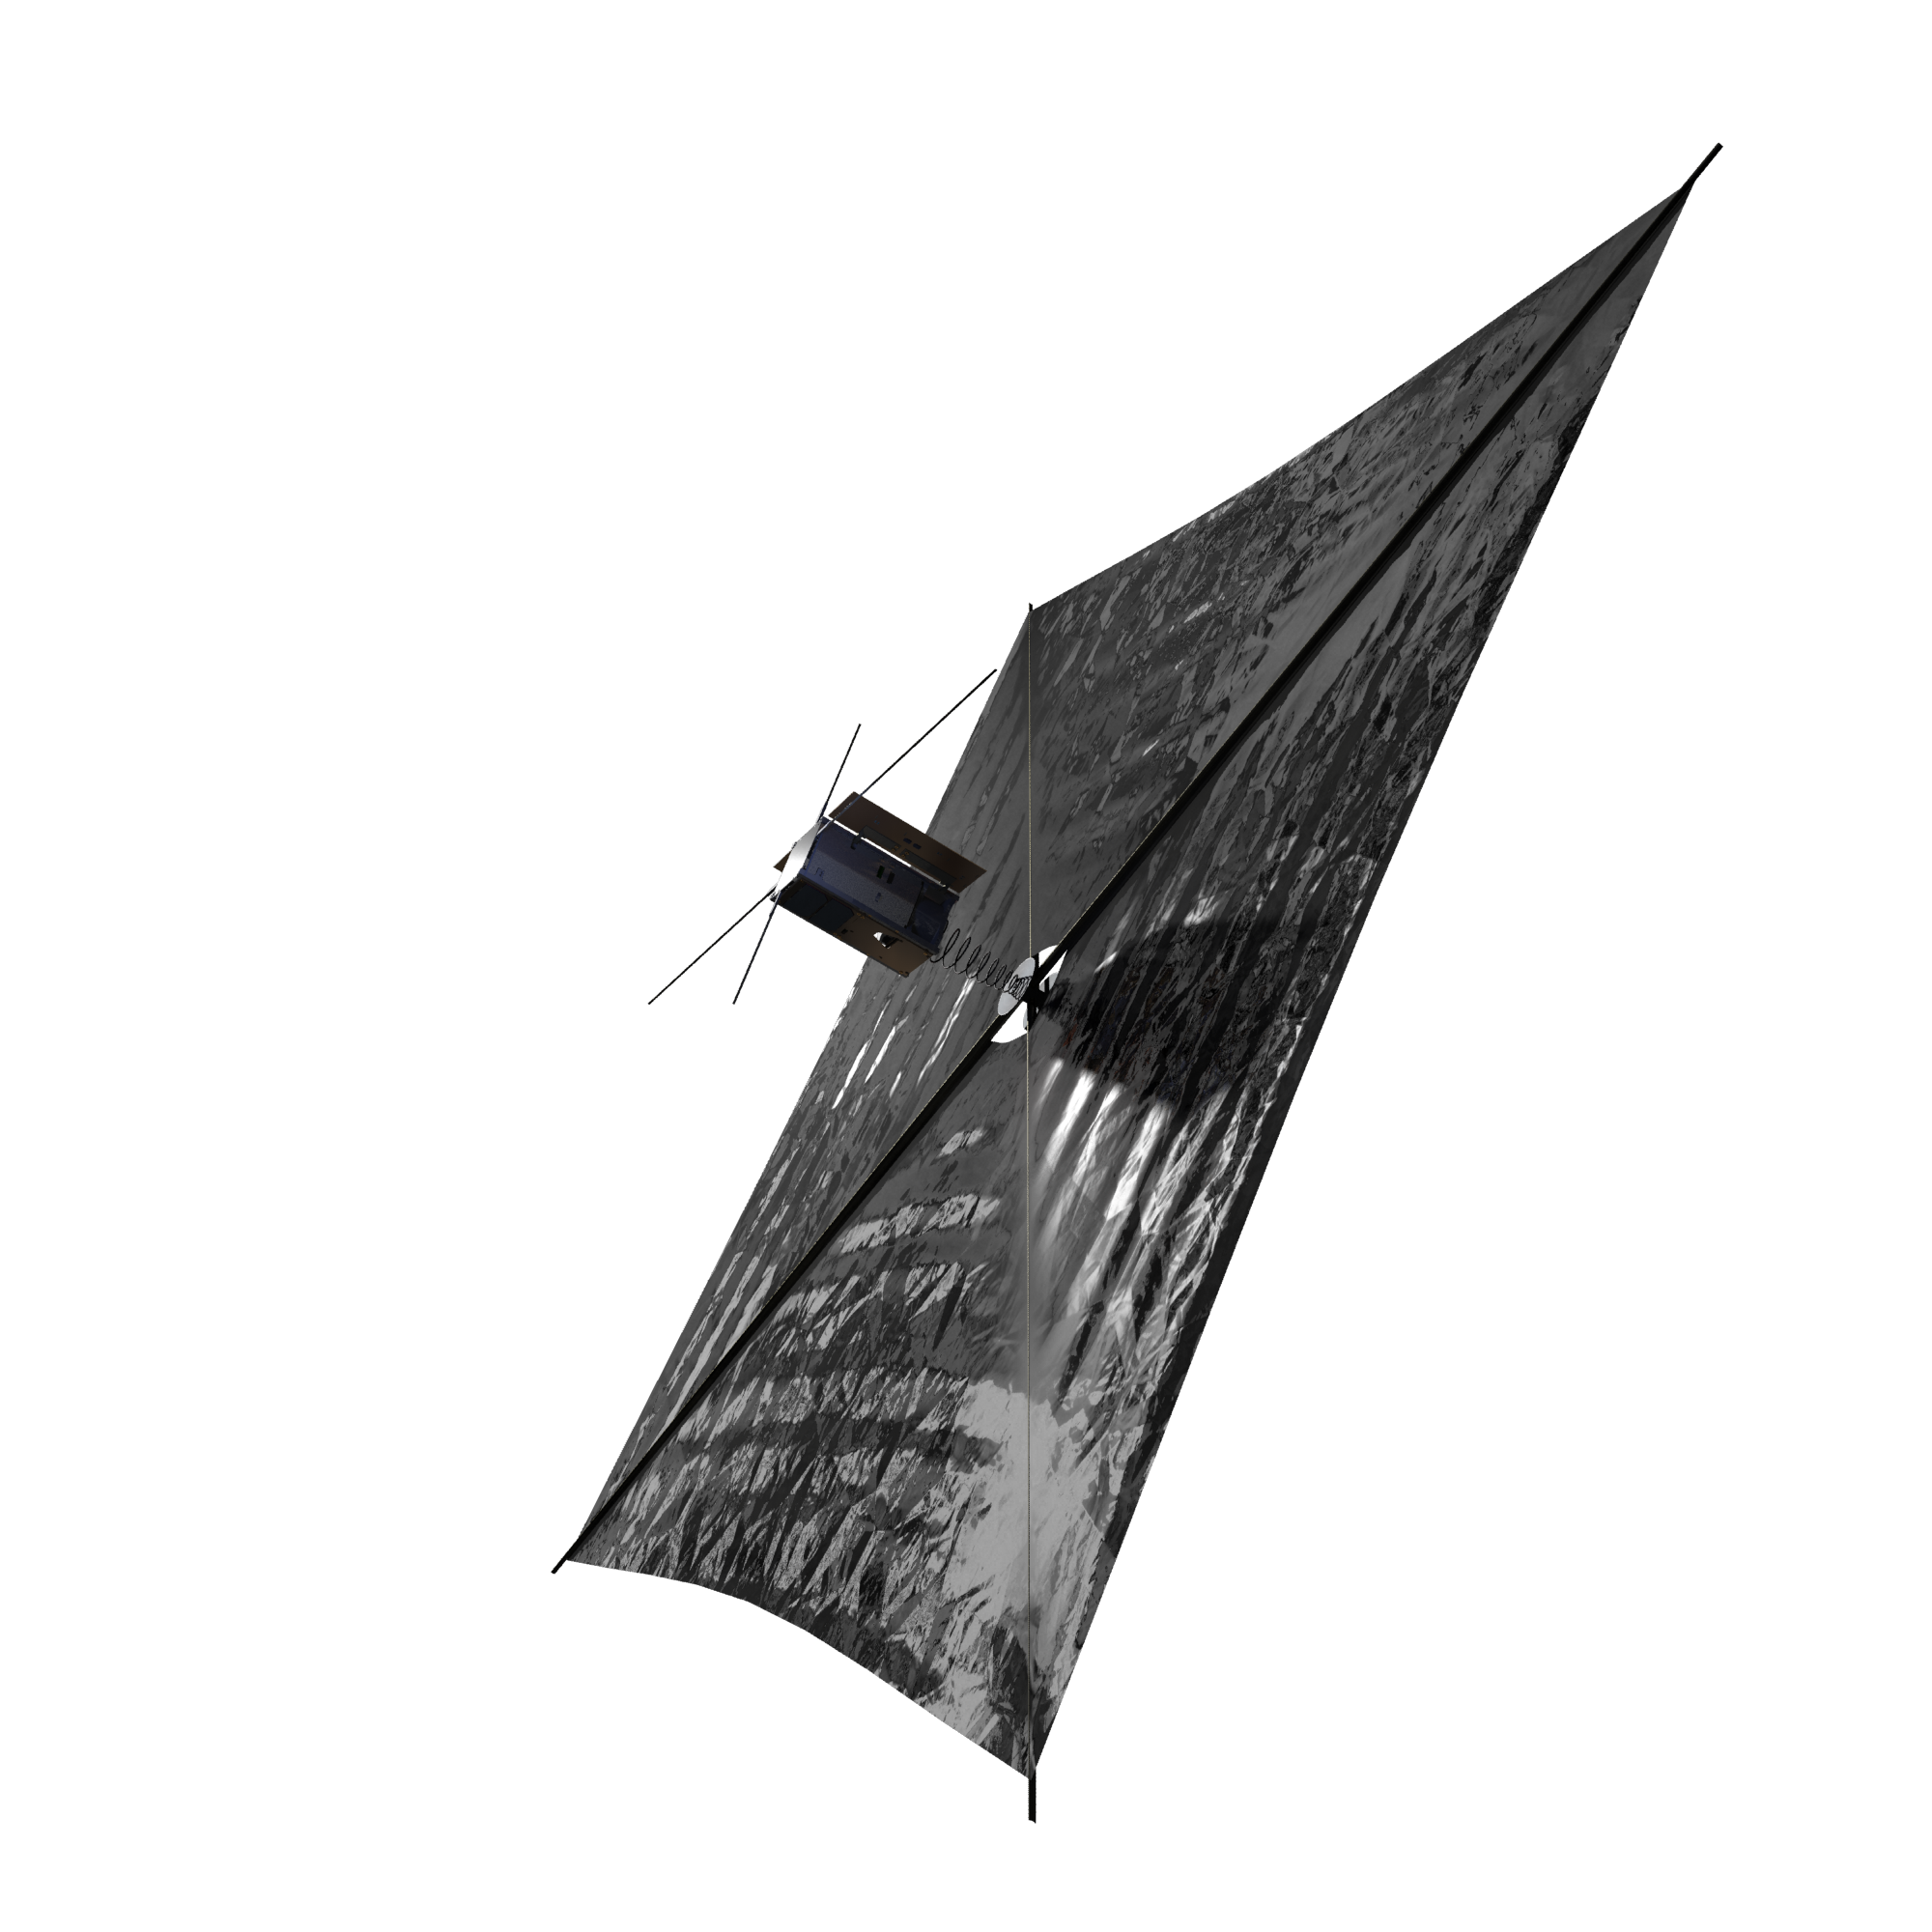
\includegraphics[width=0.7\paperwidth]{img/PW-Sat2_render_02.png}
		\caption{PW-Sat2 with opened sail (by M. Świetlik)}
		\label{PW-Sat_render_sail}
	\end{figure}
	
	More information can be found in \cite{DDC_article}.
	
\subsection{Lifetime}
	Due to its primary mission PW-Sat2 mission is planned to be 40 days long. After this time deorbit sail will open, possibly causing lack of communication with satellite. Therefore sensor should be able to measure dose absorbed during 40 days on orbit.
	
\subsection{Orbit}
	PW-Sat2 in planned to be launched to sun-synchronous circular orbit of attitude $575~km$, with LTAN of $10:30$ \cite{PWSAT_MA_CDR}.
	

\subsection{Radiation analysis}
	Simulations in SPENVIS \cite{SPENVIS_URL} were performed to determine TID accumulated during PW-Sat2 mission. On fig \ref{TIDvsSheilding} dose as a function of shielding thickness was plotted.

	\begin{figure}[H]
		\centering
		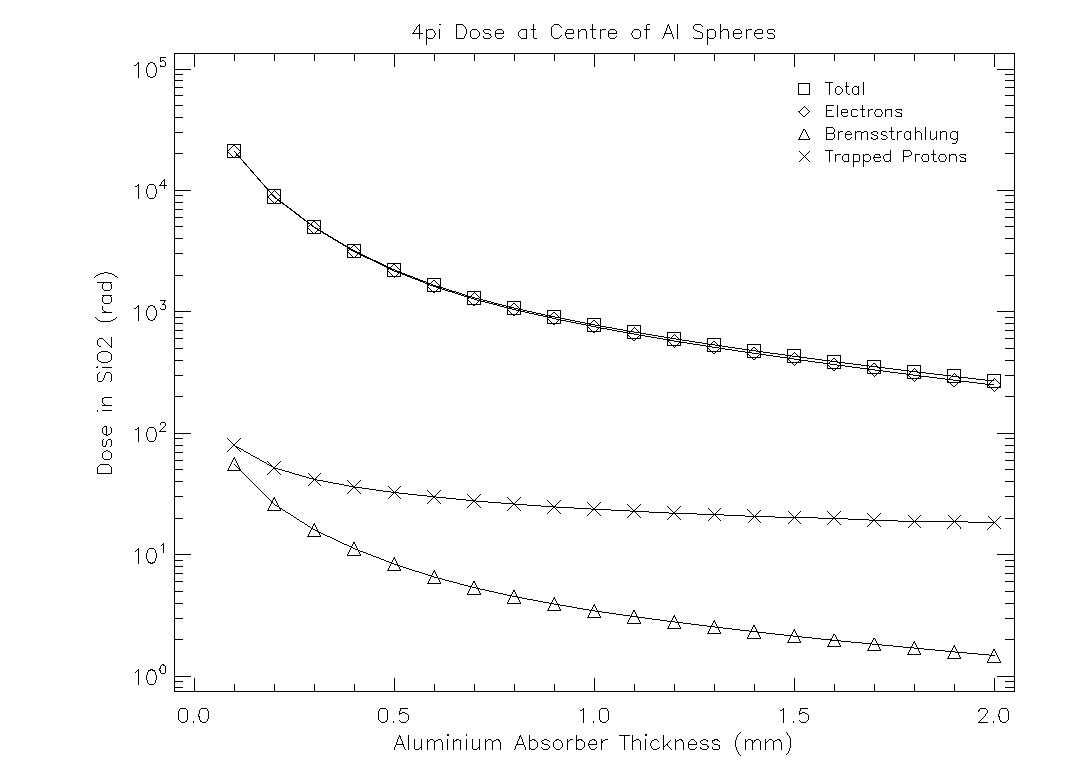
\includegraphics[width=0.7\paperwidth]{img/dose.eps}
		\caption{TID vs shielding}
		\label{TIDvsSheilding}
	\end{figure}

	Shielding of PW-Sat2 is about $1~mm$ thick (aluminium sides as well as aluminium base for solar cells - \ref{PW-Sat_render_01}). Therefore predicted dose during PW-Sat2 mission is about $1$~kRad.




\section{Sensor requirements}
	In this section sensor requirements are presented.

\subsection{Range}
	Total range of the sensor should be more than predicted dose ($>~1$~kRad). With $300\%$ reserve: designed sensor should have range of more than $3$~kRad.
	
\subsection{Accuracy \& resolution}
	Sensor should be able to detect low radiation doses. Its resolution should be lower than $0.1$~kRad, with accuracy of less than $0.5$~kRad.




\section{Applicable standards}
	The sensor should comply to ECSS \cite{ECSS_URL} standards. They are required from launch provider, as well as describing good practices during space product development.
	
	ESCIES \cite{ESCIES_URL} provide valuable knowledge about components qualifications, testing and verification.



\section{Electrical requirements}
	Sensor will be placed on-board of PW-Sat2. Therefore it should comply to its' standards - power supplies, communication interfaces etc.
	
\subsection{Electronics stack}
	Modules on PW-Sat2 are connected in PC-104 stack structure as shown on figure \ref{PW-Sat2_stack}. Is is placed inside structure and consists of (from the top):
	\begin{itemize}
		\item Payload module (PLD)
		\item On-Board Computer (OBC)
		\item Attitude Determination and Control Subsystem (ADCS)
		\item Electrical Power System (EPS)
		\item battery module (ACC)
		\item communication transceiver (COMM)
		\item antennas module (ANT)
	\end{itemize}

	\begin{figure}[H]
		\centering
		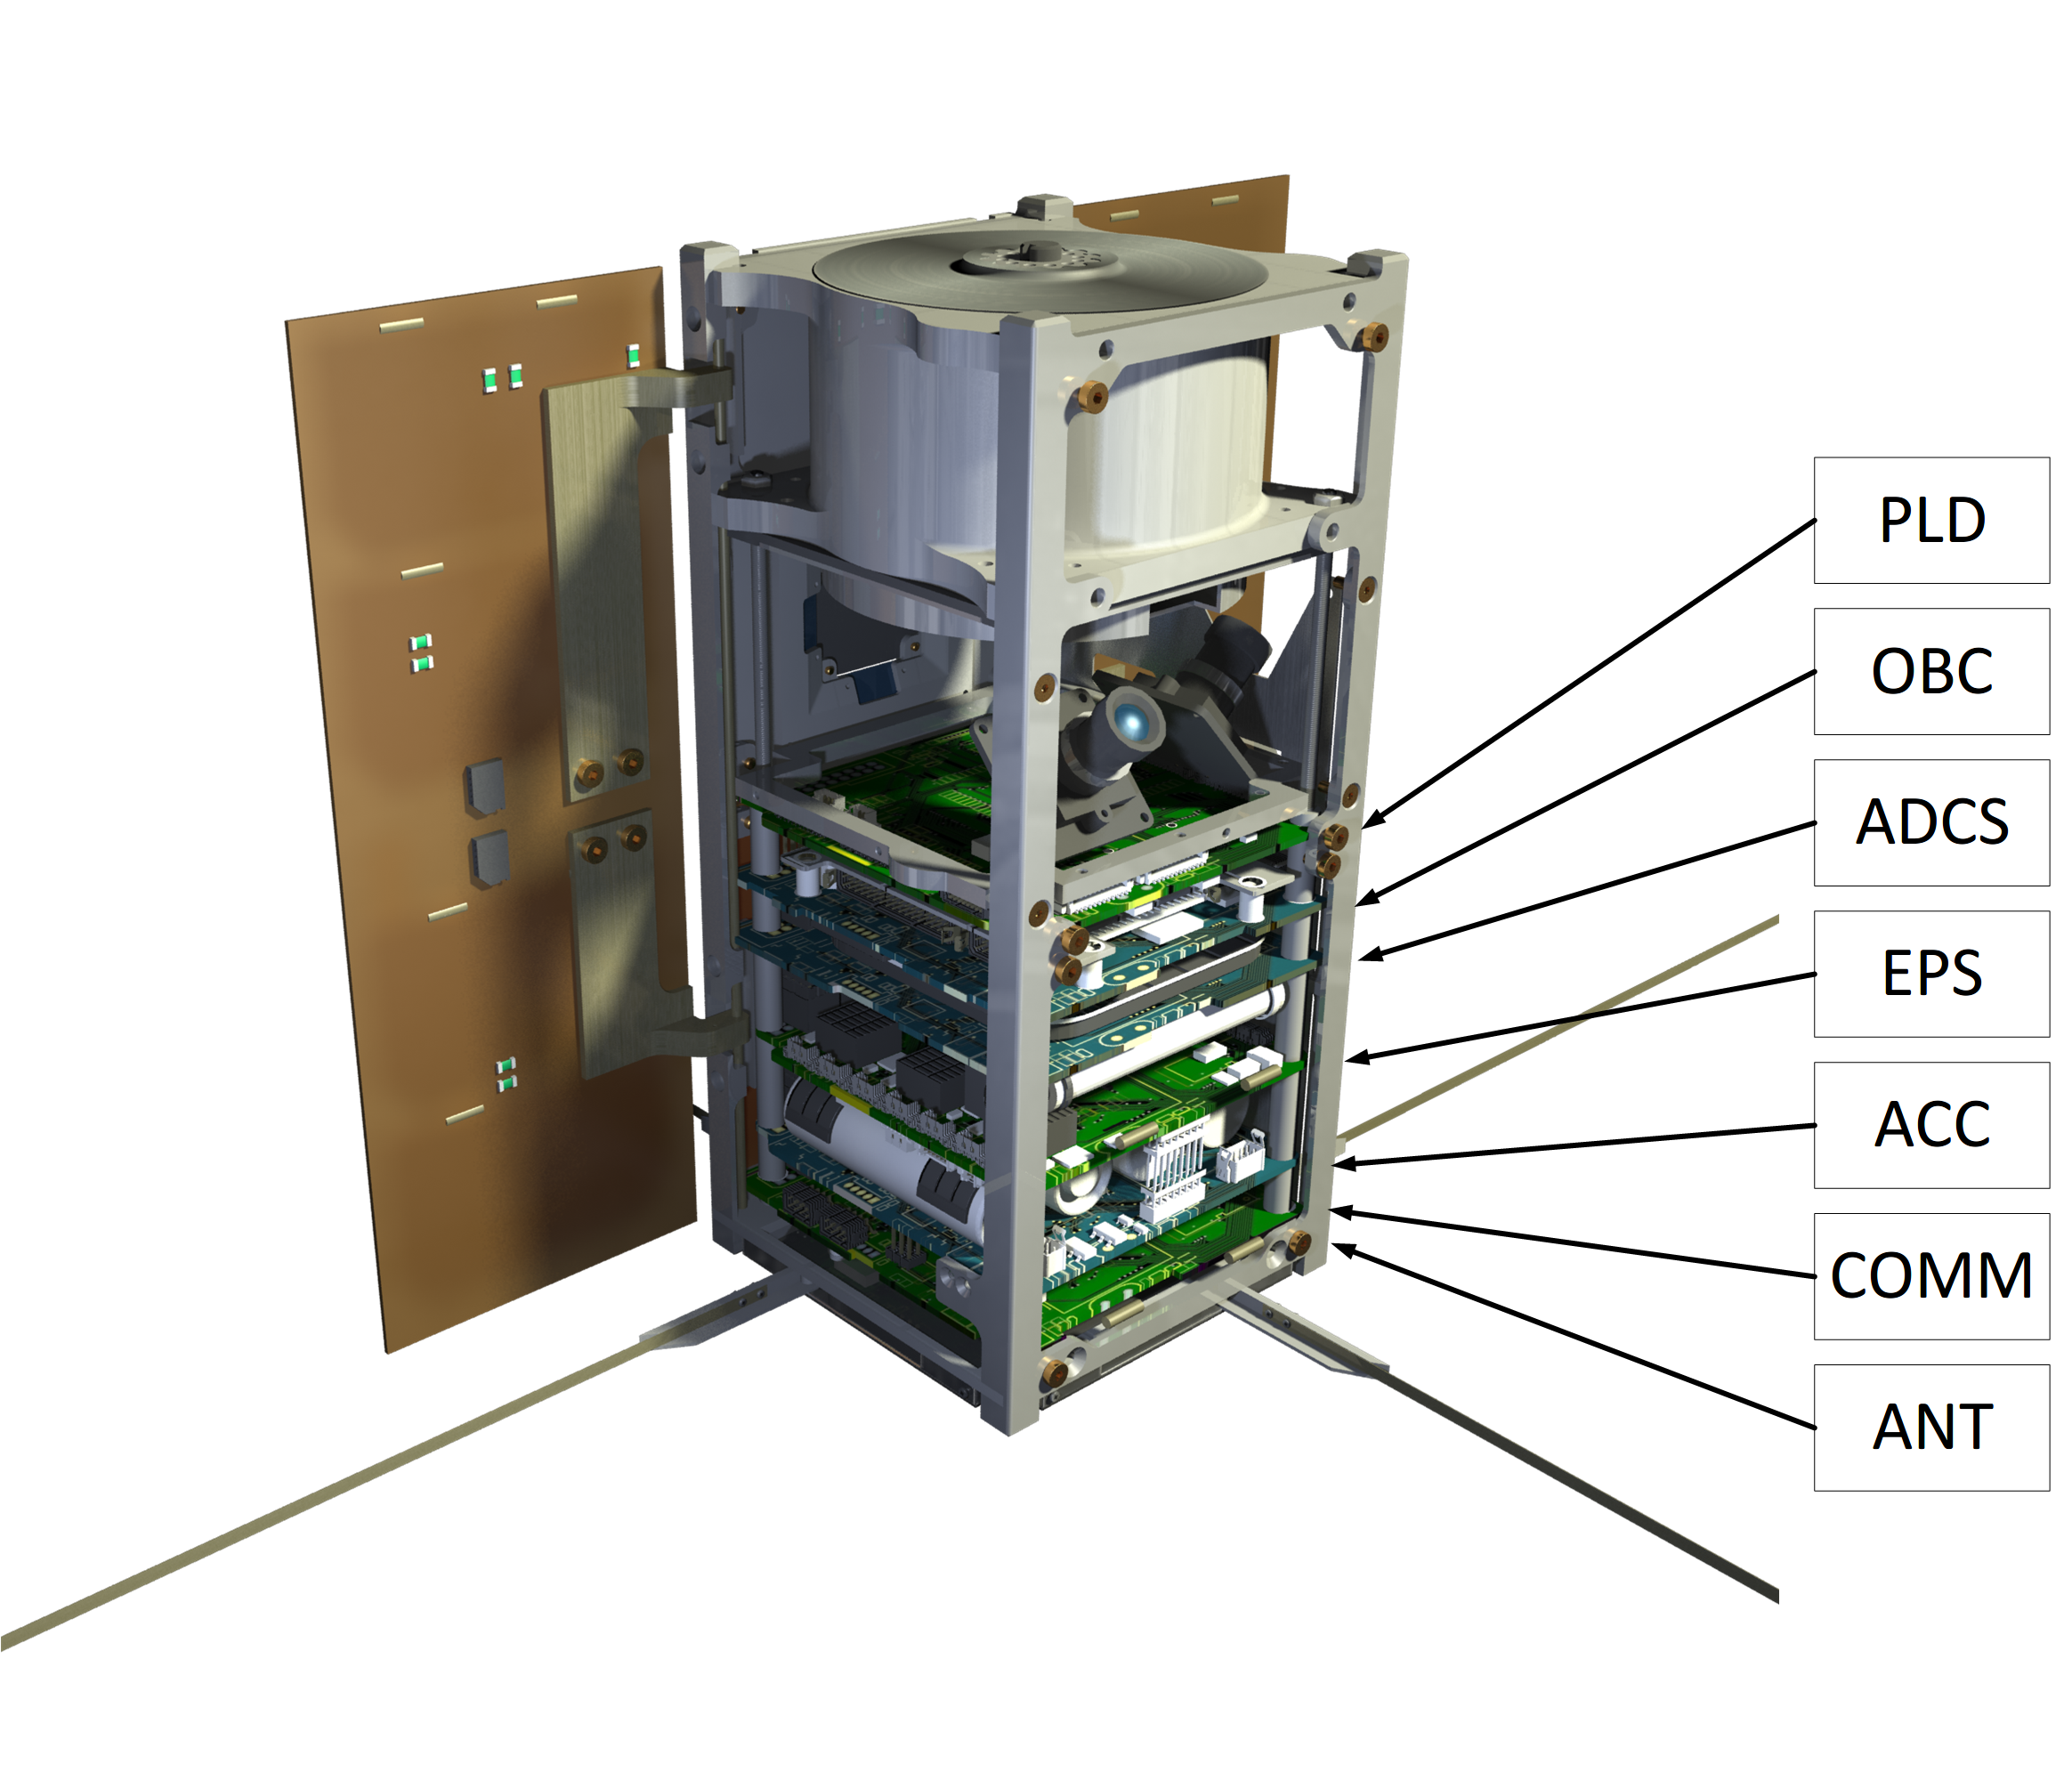
\includegraphics[width=0.7\paperwidth]{img/PW-Sat2-stack.png}
		\caption{PW-Sat2 electronics stack}
		\label{PW-Sat2_stack}
	\end{figure}


	Sensor will be placed on Payload board, on the top of PC-104 stack. It will be placed on its PCB, described in \ref{PCB_description}. It will be one of sensors on this board, connected to PC-104 stack.
	
	
\subsection{PC-104 connector}
	PLD board is connected to OBC with PC-104 connector. Pinout is shown on figure \ref{PC104_PLD}.
	
	\begin{figure}[H]
		\centering
		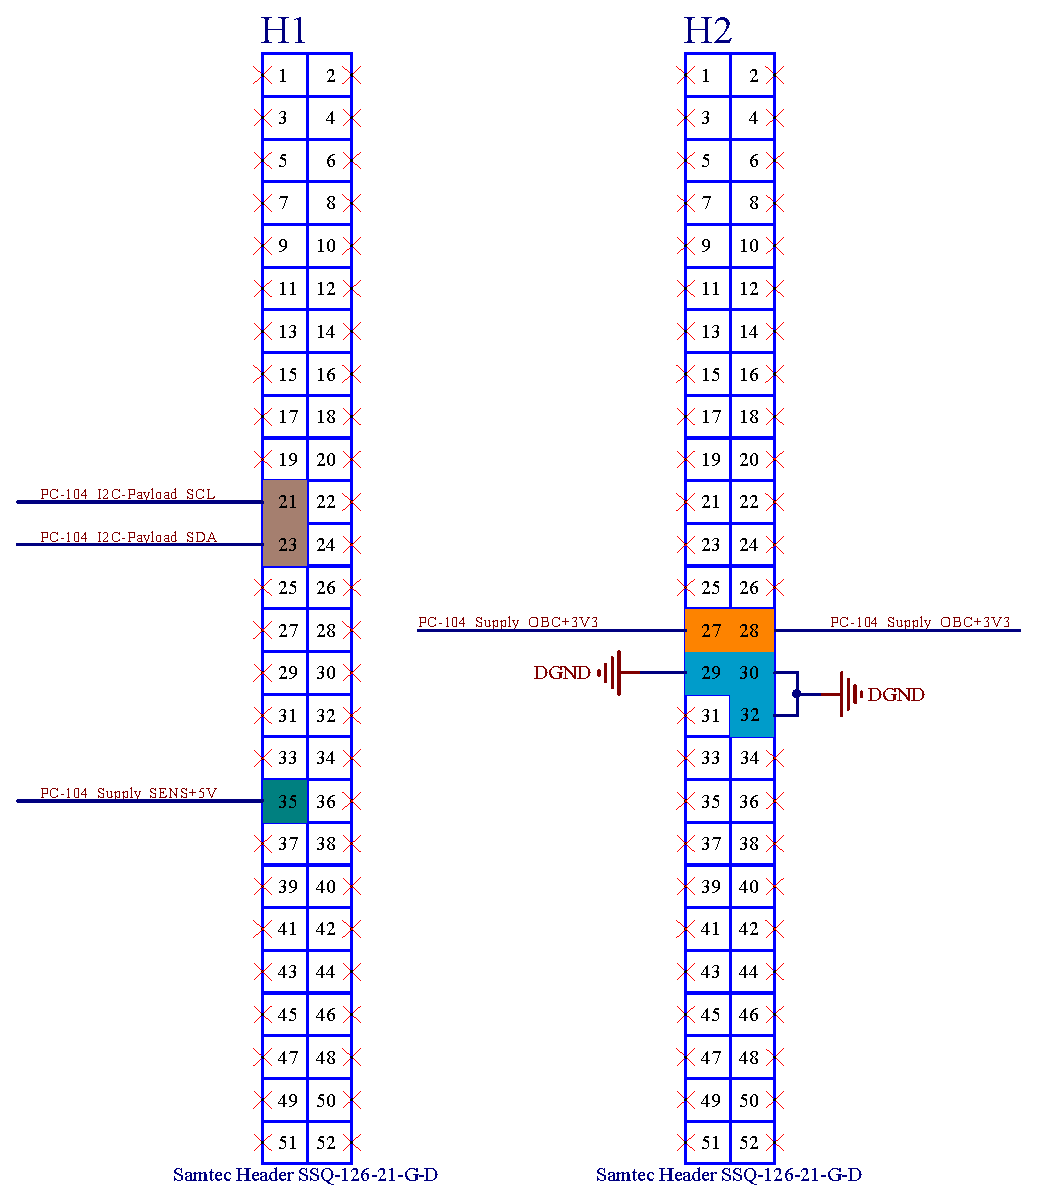
\includegraphics[width=0.5\paperwidth]{img/PC-104.eps}
		\caption{PC-104 connector to PLD board}
		\label{PC104_PLD}
	\end{figure}

	Connector consists of:
	\begin{itemize}
		\item $I^2C$ bus, connected directly to MCU on OBC,
		\item OBC $3.3$~V line, connected directly to MCU on OBC,
		\item SENS $5$~V line, powered when sensor is enabled by OBC.
	\end{itemize}

\subsection{Power}
	As mentioned earlier, the power for the sensor is $+5$~V, activated whenever sensor should be accessed by OBC. 
	
	Power line is controlled and protected by Latchup-Current Limiter FPF2700 placed on EPS board. Therefore additional latchup protection in not necessary in this design. The sensor is enabled and disabled by EPS on OBC command. Having this in mind forces the design to be immune to immediate shutdowns. 
	
\subsection{Data interface}
	The sensor is connected to OBC via $I^2C$ interface. OBC on this bus is master - and sensor should be one of slaves. PLD board can be disabled, therefore it should provide isolation of $I^2C$ bus when it is powered off.
	
\subsection{Radiation immunity}
	Design should be itself immune to radiation. For PW-Sat2 threshold of $10$~kRad was chosen for all COTS components. Every used semiconductor should have passed appropriate radiation tests as described in \cite{ESCIES_TID_test_method}.

\subsection{Electromagnetic compatibility}
	On board PW-Sat2 is a communication module transmitting $0.5$~W of power on frequency of $435.02$~MHz. Sensor should be immune to radiated emission from it, as well as conducted noise coupled into power lines.

\subsection{Reliability of components}
	This sensor is not a critical part of the satellite. But, reliable components should be used to ensure proper results. 
	
	Every used component should have failure rate of $0.01\%$ or lower.


\section{Mechanical requirements}
	In this chapter design constrains and mechanical requirements of Falcon9 are presented. Launcher requirements were taken from \cite{Falcon9_user_manual}.
	
\subsection{PCB}
\label{PCB_description}
	PCB of PLD board is standard 4-layer FR4 board with stack shown on figure \ref{PLD_PCB_stack}. Its dimensions are shown on \ref{PLD_PCB_size}, but design is forced to take much less space. For this sensor limits are $3x3$~cm double sided.

	\begin{figure}[H]
		\centering
		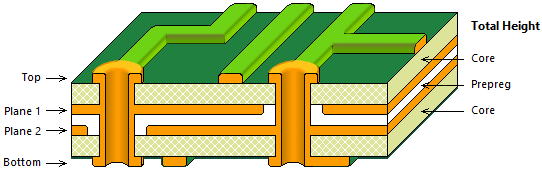
\includegraphics[width=0.5\paperwidth]{img/PLD_PCB_stack.png}
		\caption{PLD board PCB stack}
		\label{PLD_PCB_stack}
	\end{figure}	

	\begin{figure}[H]
		\centering
		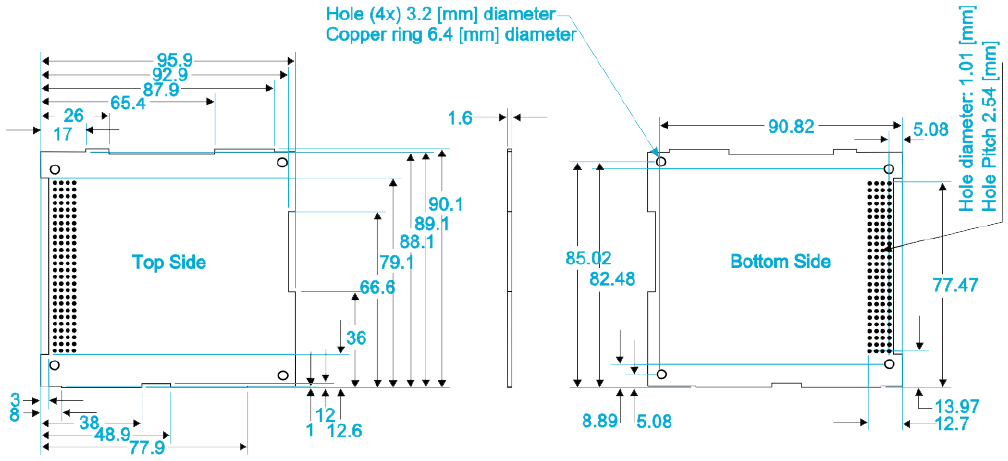
\includegraphics[width=0.7\paperwidth]{img/PC104_PLD_size.png}
		\caption{PC-104 size}
		\label{PLD_PCB_size}
	\end{figure}	
		
	

\subsection{Outgassing}
	Every used component should be able to work in vacuum. Outgassing of components should be known due to required vacuum tests before launch.
	
\subsection{Vibration}
	During rocket launch large vibrations occur on payload, therefore it should be immune to it. In case of any heavy electronic components appropriate glue should be applied to prevent joint cracks.
	\begin{figure}[H]
		\centering
		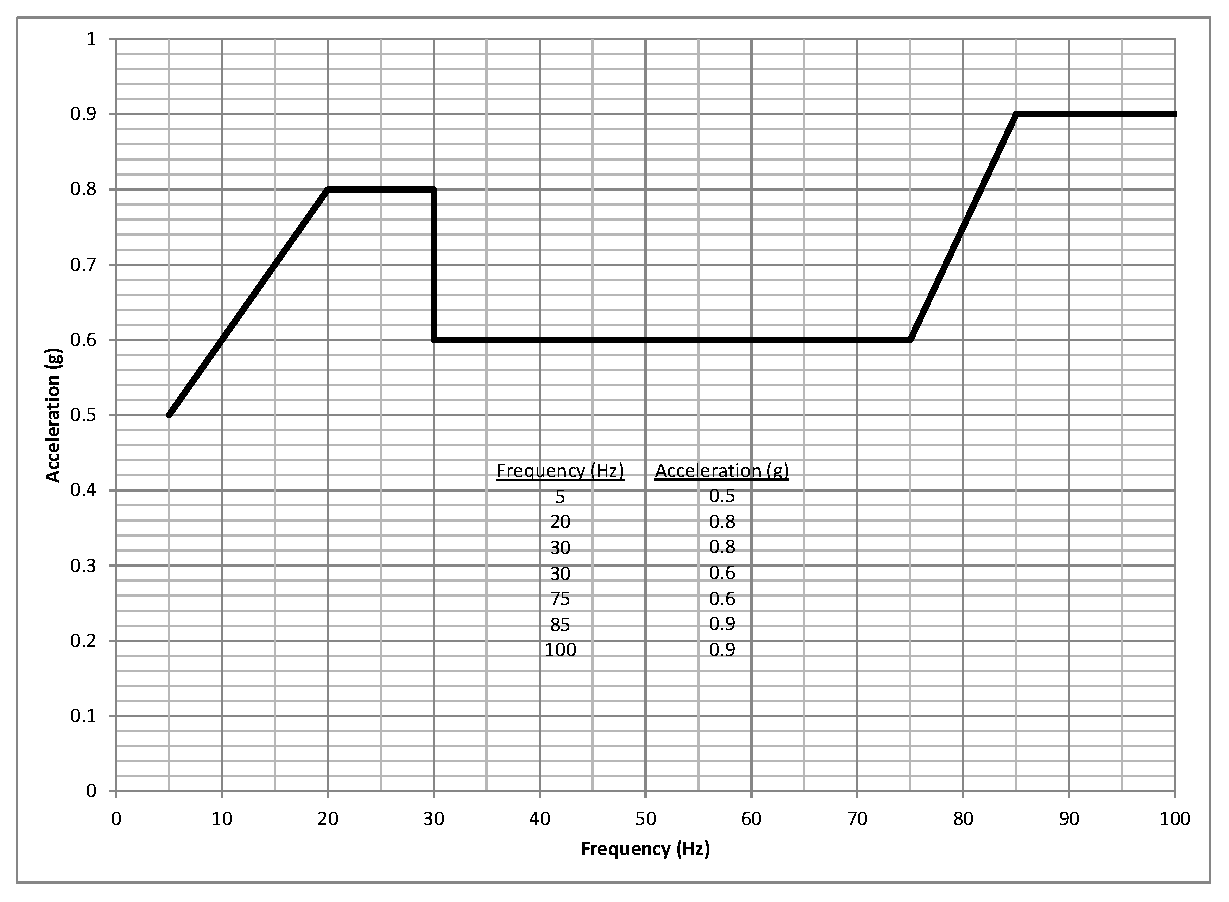
\includegraphics[width=0.5\paperwidth]{img/Falcon9_vibration.eps}
		\caption{Falcon9 maximum axial equivalent sine environment. Source: \cite{Falcon9_user_manual}}
		\label{Falcon9_vibration}
	\end{figure}	


\subsection{Operation temperature}
	The sensor should work in every operational case satellite can be. Simulations were performed to find bounds of possible temperature range inside satellite.	In \cite{PWSAT_TCS_CDR} results are presented. 
	
	In shorthand:
	\begin{itemize}
		\item Minimum operational temperature: $-30^\circ C$
		\item Maximum operational temperature: $60^\circ C$
	\end{itemize}


\subsection{Thermal cycles}
	Or PW-Sat2 orbit sun illumination is changing every $\approx 90min$. Therefore large number of thermal cycles are applied to On-Board electronics, which can cause joint cracks as well as component failures. 
	
	As described in \cite{ECSS_Q_ST_70_04C} the sensor should pass thermal cycle tests: $100$ times from $- (100 \pm 5)^\circ C$ to $(100 \pm 5)^\circ C$ in vacuum environment. Test procedure is shown on \ref{thermal_tests}.
	
	\begin{figure}[H]
		\centering
		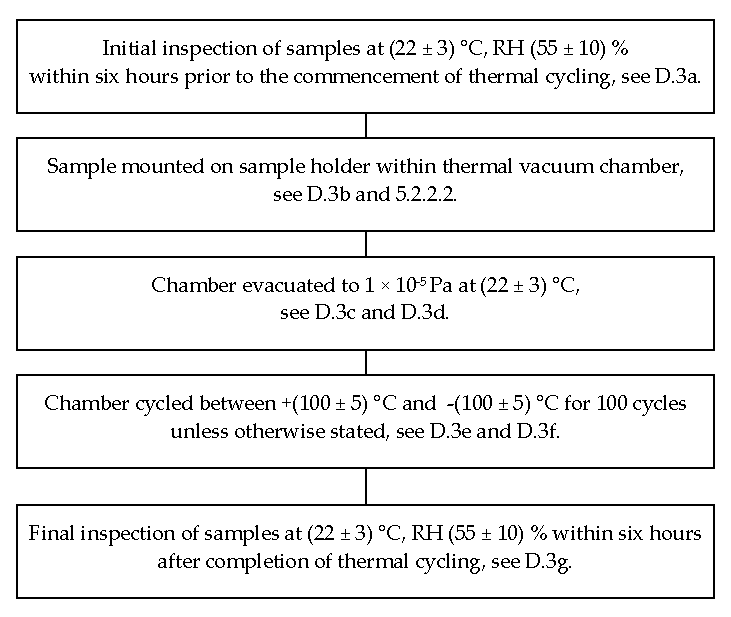
\includegraphics[width=0.5\paperwidth]{img/thermal_cycles.eps}
		\caption{Thermal cycles test procedure. Source: \cite{ECSS_Q_ST_70_04C}}
		\label{thermal_tests}
	\end{figure}
